%%%%%%%%%%%%%%%%%%%%%%%%%%%%%%%%%%%%%%%%%%%%%%%%%%%
%% LaTeX book template                           %%
%% Author:  Amber Jain (http://amberj.devio.us/) %%
%% License: ISC license                          %%
%%%%%%%%%%%%%%%%%%%%%%%%%%%%%%%%%%%%%%%%%%%%%%%%%%%

\documentclass[a4paper,11pt]{book}
\usepackage[T1]{fontenc}
\usepackage[utf8]{inputenc}
\usepackage{xeCJK}          %导入xeCJK包
\usepackage{lmodern}
%%%%%%%%%%%%%%%%%%%%%%%%%%%%%%%%%%%%%%%%%%%%%%%%%%%%%%%%%
% Source: http://en.wikibooks.org/wiki/LaTeX/Hyperlinks %
%%%%%%%%%%%%%%%%%%%%%%%%%%%%%%%%%%%%%%%%%%%%%%%%%%%%%%%%%
\usepackage{hyperref}
\usepackage{graphicx}
\usepackage[english]{babel}

%%%%%%%%%%%%%%%%%%%%%%%%%%%%%%%%%%%%%%%%%%%%%%%%%%%%%%%%%%%%%%%%%%%%%%%%%%%%%%%%
% 'dedication' environment: To add a dedication paragraph at the start of book %
% Source: http://www.tug.org/pipermail/texhax/2010-June/015184.html            %
%%%%%%%%%%%%%%%%%%%%%%%%%%%%%%%%%%%%%%%%%%%%%%%%%%%%%%%%%%%%%%%%%%%%%%%%%%%%%%%%
\newenvironment{dedication}
{
   \cleardoublepage
   \thispagestyle{empty}
   \vspace*{\stretch{1}}
   \hfill\begin{minipage}[t]{0.66\textwidth}
   \raggedright
}
{
   \end{minipage}
   \vspace*{\stretch{3}}
   \clearpage
}

%%%%%%%%%%%%%%%%%%%%%%%%%%%%%%%%%%%%%%%%%%%%%%%%
% Chapter quote at the start of chapter        %
% Source: http://tex.stackexchange.com/a/53380 %
%%%%%%%%%%%%%%%%%%%%%%%%%%%%%%%%%%%%%%%%%%%%%%%%
\makeatletter
\renewcommand{\@chapapp}{}% Not necessary...
\newenvironment{chapquote}[2][2em]
  {\setlength{\@tempdima}{#1}%
   \def\chapquote@author{#2}%
   \parshape 1 \@tempdima \dimexpr\textwidth-2\@tempdima\relax%
   \itshape}
  {\par\normalfont\hfill--\ \chapquote@author\hspace*{\@tempdima}\par\bigskip}
\makeatother


%定义习题主题
\newtheorem{question}{习题}[section]

%%%%%%%%%%%%%%%%%%%%%%%%%%%%%%%%%%%%%%%%%%%%%%%%%%%
% First page of book which contains 'stuff' like: %
%  - Book title, subtitle                         %
%  - Book author name                             %
%%%%%%%%%%%%%%%%%%%%%%%%%%%%%%%%%%%%%%%%%%%%%%%%%%%

% Book's title and subtitle
\title{\Huge \textbf{电动力学题解}
\\ \huge 往年考试例题与解答 \footnote{吉林大学物理学院电动力学课程}}
% Author
\author{\textsc{王大可}\thanks{\url{www.example.com}} \and\textsc{小锡}\thanks{\url{www.example.com}}}


\begin{document}

\frontmatter
\maketitle

%版权声明
\begin{center}
王大可与小锡拥有版权©2018。保留所有权力。\\
\begin{figure}[h!]
\centering

\includegraphics[scale=1]{images/by-nc-sa.png}
\end{figure}
本作品采用知识共享 署名-非商业性使用-相同方式共享 4.0 国际 许可协议进行许可。要查看该许可协议,可访问 \href{https://creativecommons.org/licenses/by-nc-sa/4.0/}{https://creativecommons.org/licenses/by-nc-sa/4.0/} 或者写信到 Creative Commons, PO Box 1866, Mountain View, CA 94042, USA。
\end{center}

%%%%%%%%%%%%%%%%%%%%%%%%%%%%%%%%%%%%%%%%%%%%%%%%%%%%%%%%%%%%%%%
% Add a dedication paragraph to dedicate your book to someone %
%%%%%%%%%%%%%%%%%%%%%%%%%%%%%%%%%%%%%%%%%%%%%%%%%%%%%%%%%%%%%%%
\begin{dedication}
献给可爱的学妹们
\end{dedication}

%%%%%%%%%%%%%%%%%%%%%%%%%%%%%%%%%%%%%%%%%%%%%%%%%%%%%%%%%%%%%%%%%%%%%%%%
% Auto-generated table of contents, list of figures and list of tables %
%%%%%%%%%%%%%%%%%%%%%%%%%%%%%%%%%%%%%%%%%%%%%%%%%%%%%%%%%%%%%%%%%%%%%%%%
\renewcommand{\contentsname}{目录}%将contents改为中文目录
\tableofcontents

\mainmatter

%%%%%%%%%%%
% Preface %
%%%%%%%%%%%
\chapter*{前言}

本书作为吉林大学物理学院电动力学课程的历年试题解答,力求详细,准确且便于理解的给出习题答案。本书主要基于吉大物院电动力学课本,此外非常推荐去看郭硕鸿先生以及格里菲斯先生的电动力学教材。



%%%%%%%%%%%%%%%%
% NEW CHAPTER! %
%%%%%%%%%%%%%%%%
\chapter{往年试题}

\begin{chapquote}{\textit{Genesis 1:3}}
``And God said 
$$\nabla \cdot \mathbf{D}=\rho$$
$$\nabla \times \mathbf{E} =- \frac{\partial \mathbf{B}}{\partial t}$$
$$\nabla \cdot \mathbf{B} =0$$
$$\nabla \times \mathbf{H}=\mathbf{J}+\frac{\partial \mathbf{D}}{\partial t}$$
and there was light
''
\end{chapquote}

\section{电磁现象的基本规律}
对应电动力学课本第二章,占分20分左右。

\begin{question}
写出电磁现象的基本规律,其中包括真空中的Maxwell方程组,电荷守恒定律,洛仑兹力公式,介质的电磁性质方程及电磁场的边界条件。
\end{question}

\begin{question} 
从毕奥-萨伐尔定律出发推导出磁场的散度。
\end{question}

\begin{question} 
从基本的麦克斯韦(Maxwell)方程组出发,推出静电场的基本方程和边界条件。
(需说明静电场的特殊条件,引入电势,将静电场的方程和边界条件用电势来表示)
\end{question}

\begin{question} 
证明:通过任意闭合曲面的自由电流和位移电流的总量为零。
\end{question}

\begin{question} 
一长直导线半径为a,电导率为$\rho$,导线中的电流强度为I,设导线表面带有正电荷$\delta$
,计算导体表面外侧的能流密度矢量,并证明单位时间内流入长为L的一段导体的能量,恰好是L长导线的焦耳热损耗。
\end{question}

\begin{question}
叙述法拉第电磁感应定律与楞次定律;由法拉第定律推出变化磁场产生的电场的旋度;麦克斯韦对变化磁场产生的电场的散度做了什么假定?导出电荷产生的电场和变化磁场产生的电场的总电场的散度和旋度。
\end{question}

\begin{question}
1. 从库仑定律可以推出高斯定理,从高斯定理是否可以推出库仑定律?
2. 从毕奥-萨伐尔定律可以推出安培环路定理,安培环路定理是否能代替毕奥-萨伐尔定律?
\end{question}

\begin{question}
推出磁化电流密度与磁化强度之间的关系,并需画图说明。
\end{question}

\begin{question} 
推出束缚电荷密度与极化强度之间的关系 ,并需画图以及严谨的说明 。
\end{question}

\begin{question} 
静电场,稳定电磁场,电偶极子的电磁场以及电磁波传播的求解问题是普遍的麦克斯韦方程组在特定物理条件下的求解问题。分别写出这些物理条件。
\end{question}

\begin{question} 
(1)说明什么是电磁感应现象。(2)陈述法拉第电磁感应定律和楞次定律,并结合这两个定律给出统一的数学表达式。(3)指出动生电动势和感生电动势的区别。(4)推出变化磁场引起的电场的旋度。(5)关于变化磁场引起的电场的散度,麦克斯韦做了什么假定。
\end{question}

\begin{question} 
从麦克斯韦(Maxwell)方程组的积分形式推出磁场强度 的边界条件。
\end{question}

\begin{question} 
已知束缚电荷密度与极化强度的关系为 ,极化电流密度为 ,磁化电流密度与磁化强度的关系为 。从真空中的麦克斯韦方程组出发引入电位移矢量 和磁场强度 推出介质中的麦克斯韦方程组。
\end{question}

\begin{question} 
从库仑定律可以推出静电场的散度和旋度,那么从法拉第电磁感应定律能否推出变化磁场引起的电场的散度和旋度?为什么?
\end{question}

\section{静电场}
对应课本第三章,占分20分左右

\begin{question}
有一半径为a的导体球,原先不带电,在球外离球心为d处放一点电荷q,设导体球接地,用电像法求空间电势,球面上感应电荷密度。(要求写清楚电像法的步骤)
\end{question}

\begin{question}
在均匀外电场$E_0$中置入半径为$R_0$的导体球,导体球上带总电荷Q ,试用分离变数法求导体球外的电势。
\end{question}

\begin{question}
平行板电容器的平板间相距为d,两极间加直流电压V,
下板电势高。在下板内侧面上有一很小的半球突起,球半径为a(a=d),求电容器内的电场和半球上的电荷密度。
\begin{figure}[ht]
\centering
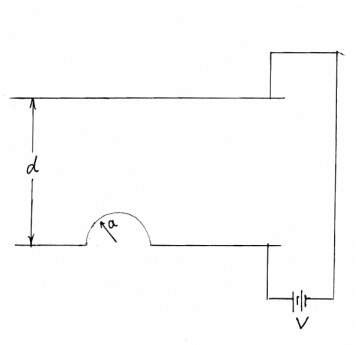
\includegraphics[height=3 cm]{images/q1_2_3.jpg}
\caption{题\thequestion}
\end{figure}

\end{question}

\begin{question}
有一半径为a的导体球,原先不带电,在球外离球心为d处放一点电荷q,设导体球接地,用电像法求空间电势,球面上感应电荷密度。(要求写清楚电像法的步骤)
\end{question}

\begin{question}
如图所示的x>0与x<0区域充满两种均匀介质,介电常数为$\varepsilon_1$与$\varepsilon_2$,在x轴上的d处有点电荷q,用电像法求空间电势。
\begin{figure}[ht]
\centering
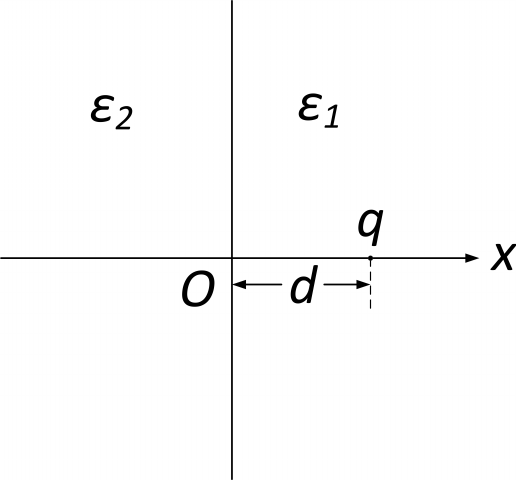
\includegraphics[height=3 cm]{images/q1_2_5.png}
\caption{题\thequestion}
\end{figure}
\end{question}

\begin{question}
求真空中带电导体球的静电能量。
\end{question}

\begin{question}
有一半径为a,介电常数为$\varepsilon$的无限长电介质圆柱,柱轴沿$\textbf{\textit{e}}_z$方向
,沿$\textbf{\textit{e}}_x$方向外加一均匀电场$E_0$,求空间电势分布。
\begin{figure}[ht]
\centering
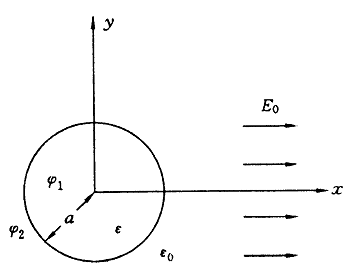
\includegraphics[height=3 cm]{images/q1_2_7.png}
\caption{题\thequestion}
\end{figure}
\end{question}

\begin{question}
一平行板电容器,板长为l,宽为b,板间距离d,如图所示,从板的左部插入一块介质,其介电常数为$\varepsilon$,插入深度为x,介质和平板之间无空隙,求介质板上受的力。略去平板电容器的边缘效应,两板间保持电位差为V。
\begin{figure}[ht]
\centering
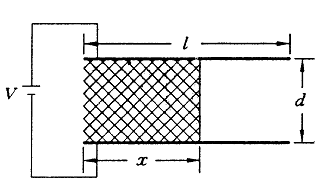
\includegraphics[height=3 cm]{images/q1_2_8.png}
\caption{题\thequestion}
\end{figure}
\end{question}

\begin{question}
如图所示 ,一半径为 a 的均匀介质球 ,介电常数为$\varepsilon_1$,介质球内带均匀自由电荷 ,电荷密度为$\rho$,介质球沉浸在介电常数为$\varepsilon_2$的无限大均匀介质中 , 在 z 方向加一均匀电场$E_0$,求球内外的电势。
\begin{figure}[ht]
\centering
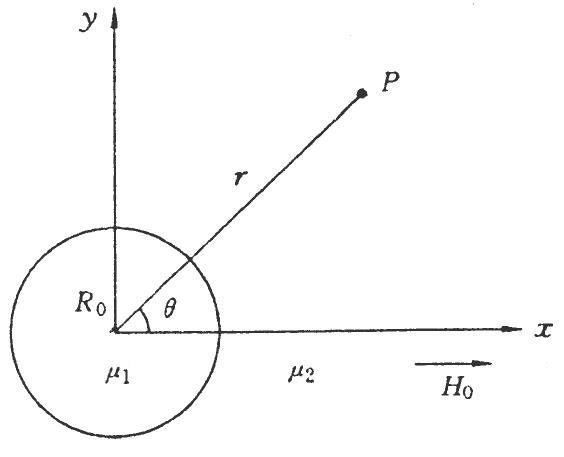
\includegraphics[height=3 cm]{images/q1_2_9.jpg}
\caption{题\thequestion}
\end{figure}
\end{question}

\begin{question}
有一均匀带电的回转椭球体 ,回转半径为a,轴半径长为c,总电量为q,计算其电偶极矩 、电四极矩以及远处的电势。
\end{question}

\begin{question}
利用格林函数方法来证明静电势的均值定理,即在无电荷的空间中的任一点的电势,等于以该点为球心任一球面上的电势的平均值。
\end{question}

\section{稳定电磁场}
对应电动力学课本第四章,占分10分左右。

\begin{question}
一半径为a的均匀带电的导体球壳,绕自身某一直径以角速度$\omega$转动,
设球上的总电量为Q(假设始终均匀分布在导体球表面),
球内外为真空,计算球内外的矢势和磁场。

\noindent(球坐标中方程$\frac{1}{r^2}\frac{\partial }{\partial r}(r^2\frac{\partial f}{\partial r})+\frac{1}{r^2 \sin\theta}\frac{\partial }{\partial \theta}(\sin\theta\frac{\partial f}{\partial \theta})-\frac{f}{r^2\sin^2\theta}=0$的一般解为:$f=\sum_{n=0}^{\infty }(b_nr^n+\frac{a_n}{r^{n+1}})P_n^{(1)}(\cos\theta)$
 ,其中一阶连带勒让德函数$P_n^{(1)}(\cos\theta)=(1-x^2)^{1/2}\frac{\mathrm{d}P_n }{\mathrm{d} x}$)
 \end{question}
 
\begin{question}
一半径为a的均匀磁化介质球,其磁化强度为$\mathbf{M_0}$,求空间静磁荷密度$\rho_m$ ,磁标势及磁场强度。
\end{question}

\begin{question}
半径为a的长直圆柱导体,均匀地沿轴方向通过恒定电流I,导体的磁导率为$\mu_1$ ,周围介质的磁导率为$\mu_2$,求矢势$\mathbf{A}$。

\noindent 可能用到的公式:柱坐标系中,

\noindent 对于标量$\phi$有:$\nabla^2\phi=\frac{1}{r}\frac{\partial }{\partial r}(r\frac{\partial \phi}{\partial r})+\frac{1}{r^2 }\frac{\partial^2 \phi}{\partial \theta^2}+\frac{\partial^2\phi}{\partial z^2}$ 

\noindent 对于矢量$\mathbf{A}$有:$\nabla \times \mathbf{A}=[\frac{1}{r}\frac{\partial A_z}{\partial \theta}-\frac{\partial A_\theta}{\partial z}]\textbf{\textit{e}}_r+[\frac{\partial A_r}{\partial z}-\frac{\partial A_z}{\partial r}]\textbf{\textit{e}}_\theta+\frac{1}{r}[\frac{\partial}{\partial r}(rA_\theta)-\frac{\partial A_r}{\partial \theta}]\textbf{\textit{e}}_z$
\begin{figure}[ht]
	\centering
	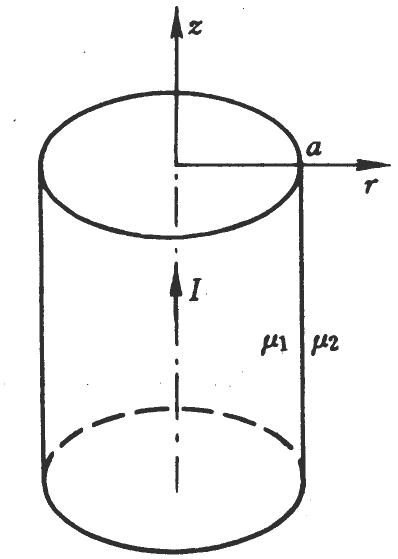
\includegraphics[height=3 cm]{images/q3_1.png}
	\caption{题1.3.3}
\end{figure}
\end{question}

\begin{question}
如图所示,一无限长的磁导率为$\mu_1$的介质圆柱,半径为$R_0$,置于磁导率为$\mu_2$的磁介质中,
在垂直于柱轴方向加一均匀静磁场$\mathbf{H_0}$,求柱内、外磁场分布。

\noindent(在柱坐标系中,$\nabla^2 \phi(r,\theta)=0$的通解为: 
$\phi=c_0 \ln r+d_0+\sum_{n=1}^{\infty}(a_n \cos n\theta+b_n \sin n\theta)(c_nr^n+d_nr^{-n})$,
其中$c_0,d_0,a_n,b_n,c_n,d_n$为常数。)
\begin{figure}[ht]
	\centering
	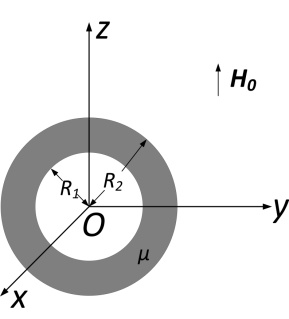
\includegraphics[height=3 cm]{images/q3_2.jpg}
	\caption{题1.3.4}
\end{figure}
\end{question}

\begin{question}
如图所示,有一内、外半径分别为$R_1$和$R_2$的空心球壳,
放置在均匀磁场$\mathbf{H_0}$中,
球壳介质的磁导率为$\mu$,球壳外为真空,求空间的磁标势。
\end{question}


\begin{question}
	一半径为a的均匀带电球壳,质量为M,总电量为Q,
	绕某一直径以角速度$\omega$转动,求磁矩和旋磁比。
\end{question}

\begin{question}
一半径为 a 的均匀带电球壳 ,总电量为 Q ,
绕某一直径以角速度$\omega$转动 ,求磁场总能量 。
\end{question}

\begin{question}
在一长直导线电流$I_1$附近,有一矩形载流线圈,电流为$I_2$,
线圈和直导线的最短距离为x,夹角为$\theta$,
如图所示,计算线圈所受的力和力矩。
\begin{figure}[ht]
	\centering
	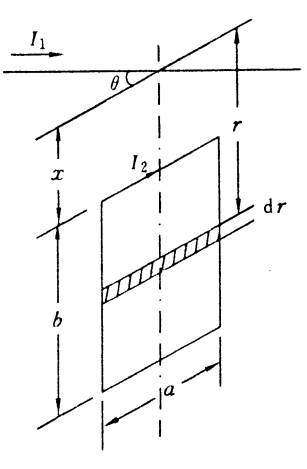
\includegraphics[height=3 cm]{images/q3_3.png}
	\caption{题1.3.8}
\end{figure}
\end{question}

\section{电磁波的辐射}
对应电动力学课本第五章,占分10分左右。

\begin{question}
这里输入题目
\end{question}

\section{电磁波的传播}
对应电动力学课本第六章,占分10分左右。

\begin{question}
这里输入题目
\end{question}

\section{狭义相对论}
对应电动力学课本第七章,占分20分左右。

\begin{question}
这里输入题目
\end{question}

\section{带电粒子和电磁场的相互作用}
对应电动力学课本第四章,占分10分左右。

\begin{question}
这里输入题目
\end{question}

\end{document}
